\documentclass{article}
\usepackage[utf8]{inputenc}
\usepackage{graphicx}
\usepackage{hyperref}

\begin{document}

\section{Nightingale}

The \textbf{common nightingale}, \textbf{rufous nightingale} or simply \textbf{nightingale} (\textit{Luscinia megarhynchos}), is a small passerine bird best known for its powerful and beautiful song. It was formerly classed as a member of the thrush family Turdidae, but is now more generally considered to be an Old World flycatcher, Muscicapidae. It belongs to a group of more terrestrial species, often called chats. \footnote{From \href{https://en.wikipedia.org/wiki/Common_nightingale}{Wikipedia}}

\subsection{Subspecies}
\begin{itemize}
  \item \textbf{Western nightingale} (\textit{L. m. megarhynchos}) - Western Europe, North Africa and Asia Minor, wintering in tropical Africa
  \item \textbf{Caucasian nightingale} (\textit{L. m. africana}) - The Caucasus and eastern Turkey to southwestern Iran and Iraq, wintering in East Africa
  \item \textbf{Eastern nightingale} (\textit{L. m. golzii}) - The Aral Sea to Mongolia, wintering in coastal East Africa
\end{itemize}

% Image:
\begin{figure}[htbp]
    \centering
    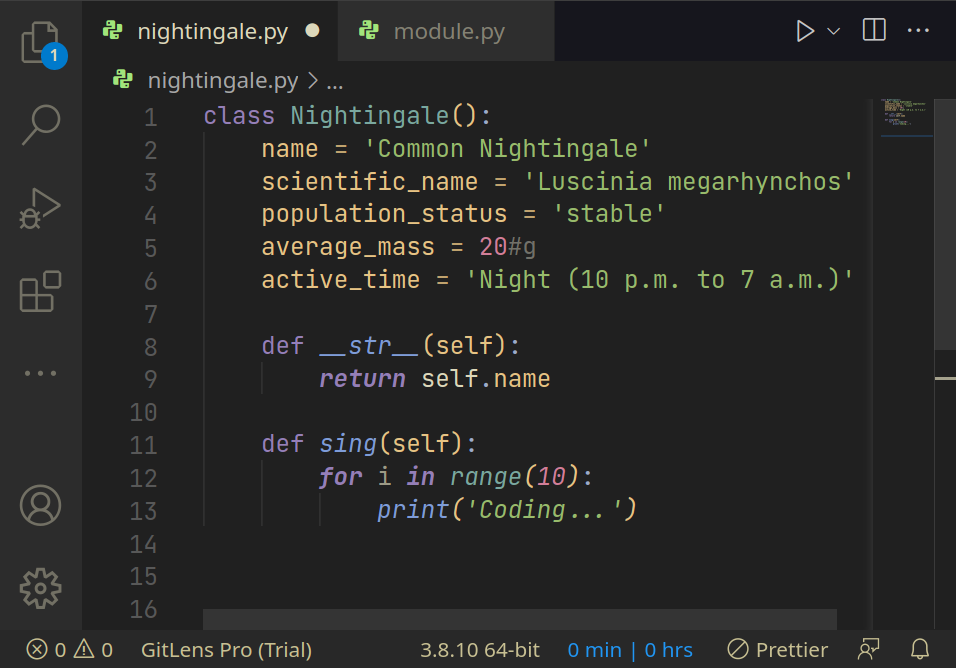
\includegraphics[width=0.5\textwidth]{nightingale.jpeg}
    \caption{Common Nightingale}
    \label{fig:nightingale}
\end{figure}


\end{document}


